\chapter{Related Work}
\label{chapter:relatedwork}

\section{Distributed Batch Systems}


Several batch systems and grid schedulers are able to schedule tasks on execution resources.  Examples of cluster schedulers that are frequently used are PBS \cite{pbstorque}, \mbox{HTCondor} \cite{litzkow1988condor}, and SLURM \cite{yoo2003slurm}.  Each scheduler is very good at resource management within a single administrative domain.  But, each of these resource managers have very limited ability to send processing to remote resources, which are typically under a separate administrative domain.  PBS and SLURM can send jobs between clusters that run the same schedulers.  HTCondor also has the ability to send processing to other clusters running HTCondor and it can also transform jobs to the language of other schedulers such as PBS and SLURM.

Grid schedulers have become more popular as the number of resources has increased.  Examples of grid schedulers are OSGMM \cite{website:osgmm} and GlideinWMS \cite{sfiligoi2008glideinwms}.  These schedulers are able to send jobs to remote resources using grid protocols.  OSGMM performs a direct grid submission to the remote resources using the GRAM  \cite{foster1999globus} interface.  GlideinWMS also submits to the GRAM interface of the cluster, but provides an overlay of HTCondor daemons on top of remote resources.  The overlay presents a consistent HTCondor interface to the computing resources for ease of use.  


\section{Distributed Storage Access}

Distributed file systems have long had their own storage access methods.  An example of this is Hadoop \cite{white2012hadoop}, a popular distributed file and processing system.  The only method to access Hadoop storage is through the Hadoop protocol.  On the Open Science Grid, the primary access methods are through file system independent middleware such as the Storage Resource Manager (SRM) \cite{shoshani2002storage} and XRootd \cite{dorigo2005xrootd}.  They provide a translation layer from system independent grid protocols and security mechanisms to the underlying storage system, such as Hadoop.  The Storage Resource Manager (SRM) is a previously popular protocol to access remote distributed filesystems.  It is a standardized protocol that allows remote, distributed access to large storage with APIs to balance transfers among many data servers.


Beyond storage access methods are storage schedulers.  These schedulers do not define a protocol to access the storage, rather they coordinate the access.  NeST \cite{bent2002flexibility} is a software-only grid aware storage scheduler.  It supports multiple transfer protocols into a storage device, including GridFTP \cite{allcock2005globus} and NFS \cite{walsh1985overview}.  Further, it provides features such as resource discovery, storage guarantees, quality of service, and user authentication.  It is layered over a distributed filesystem to provide access to it.  NeST functions as the interface and access scheduler for a storage device.  Features such as the storage guarantees and quality of service require NeST to be the only interface into the storage device, a very rare feature in today's grid storage.  Today's storage elements, such as the 3PB storage at Nebraska, include multiple interfaces to access the storage element.  Nebraska runs at least four \cite{attebury2009hadoop} methods of accessing and modifying storage, SRM \cite{shoshani2002storage}, GridFTP, XrootD, and Fuse \cite{szeredi2010fuse} mounted Hadoop.  All of these methods are required for compatibility with different access patterns and clients.  NeST could implement each of these protocols, but it would be extremely difficult to manage the storage centrally.  For example, Fuse is mounted on all 300 worker nodes.  The GridFTP and XrootD servers run on 10's of servers, with an aggregate bandwidth of 10Gbps.  Scaling quality of service and storage allocation / enforcement across all of these access methods would likely prove impossible.



\section{Data Transfer Mechanisms}

A popular consumer transfer method, Bittorrent, has been used for data transfer in computational grids by Wei et al \cite{wei2005collaborative, wei2005scheduling, wei2007towards}.  It has been shown to improve data transfer speeds when compared to traditional source and sink transfer methods, in this case FTP \cite{postel1985file}, which is very similar in architecture to GridFTP, a grid enabled FTP protocol.  The researchers did not compare performance of the bittorrent protocol when compared to modern grid transfer techniques, such as using HTTP caching.  Further, the authors do not test bittorrent transfers across network partitions that are common on the grid.  For example, a worker node from one cluster may not be able to communicate directly with another cluster.  Therefore, bittorrent may not work between clusters, but will work inside clusters.

Globus online \cite{foster2011globus} is a web interface for transferring files between sites and sharing data with other users.  It offers an intuitive web interface for bulk transfers between endpoints.  It only supports the gridftp \cite{allcock2005globus} transfer protocol, and requires GridFTP implementations at all endpoints.

There are also popular data transfer tools used on clusters such as SCP from OpenSSH \cite{openssh} and rsync.  SCP is a simple copy tool that uses the SSH protocol to transfer file from a source to a client.  Rsync is also able to copy files from a source to a client, but can also do differential copies, where only the changed portion of a directory will be copied at a time.  Both of these methods are used heavily when the data is small.  But, they both use single stream TCP in order to transfer data, which has been shown to be slower than multi-stream TCP which is used in GridFTP \cite{allcock2005globus} or BitTorrent.

\section{Data Management}

There have been previous policy frameworks for distributed storage.  These frameworks have largely been designed to move data between few large filesystems.  Therefore, the interactions are rare, but could make significant changes to the system.  In contrast, the CacheD's have frequent interactions with other agents, but each one has a minimal impact on the entire system.

Data management is different from data transfer and access in that it provides services on top of the file systems, such as meta-data storage and search capabilities.  An example of a Data management service is iRods \cite{rajasekar2010irods}.  It provides meta-data storage and querying, and rule based placements.  Further, it can handle transfers to storage resources.  iRods also has the capability to create rules and take actions on data given input.  It creates a small policy framework that upon certain actions, can execute micro-services.  This iRods policy framework is much more extensive than what we created in Chapter \ref{chapter:campusstoragepolicylanguage}.  Our framework is designed for frequent interaction between many agents acting independently.  The rules for iRods can be large, and cumbersome for simple data replication.  Further, to do anything substantial with the rules, custom code must be written.

Stork \cite{kosar2004stork} is a data placement scheduler.  It can schedule data placement and transfers to and from remote storage systems.  Stork is innovative in that it treats data transfers similar to jobs.  It will queue transfers, and checks for proper completion of the transfers.

Kangaroo \cite{thain2001kangaroo} is another storage scheduler multi-level file access system.  It allows for multiple levels of staging in order to send job output back to a storage device.  It can do this by asynchronously staging data through multiple storage devices on it's path to the destination filesystem.  The Kangaroo system only addresses output data.

DQ2 \cite{branco2008managing} and Phedex \cite{rehn2006phedex} are production transfer services for the Atlas and CMS physics experiments, respectively.  They are used to manage distributed transfers to and from sites inside the collaborations.  Additionally, they have had databases built on top of them that provide features such as combining files into datasets for easier bulk transfer management.  Both were designed for their experiments, and therefore would be very difficult to generalize for outside users.

Distributed filesystems such as Hadoop also provide a small amount of policy that can be configured.  For example, Hadoop can be configured to replicate the contents of a directory at least $X$ times.  Further, a script can be given to hadoop which it can query to create a topology of the data center, further providing control of how the data replicas are sent.  This topology script has been used by me to create a data center aware hadoop replication policy \cite{he2012hog}.

\begin{figure}[ht!]
	\centering
	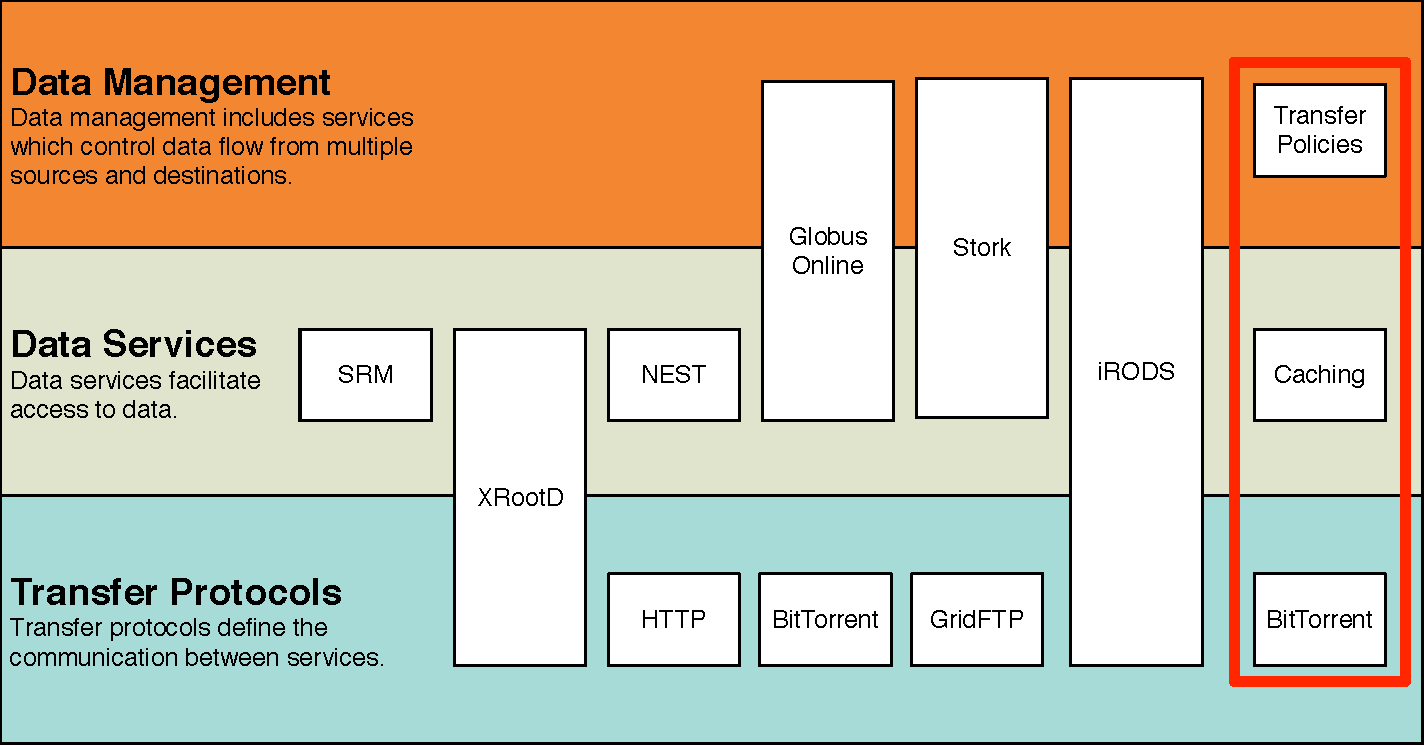
\includegraphics[width=\textwidth]{images/BackgroundStorageDiagram2.pdf}
	\caption{Background on storage technologies}
	\label{fig:backgroundstorage}
\end{figure}

Figure \ref{fig:backgroundstorage} shows an overview of the different protocols and services, and how they fit into the three categories: Data Management, Data Services, and Transfer Protocols.

\section{State of Practice in Campus Computing}
%TODO: write state of practice in campus computing

In order to illustrate the available technologies on the grid, we will begin with a typical use case.  We will then describe the technologies that could enable this computing on the grid.

\subsection{Use Case}
We will begin with a typical use case.  In this particular case, we will focus on the use of BLAST \cite{altschul1990basic}.  Blast workflows typically include the following files:

\begin{itemize}
	\item Executable
	\item Database
	\item Query Files
\end{itemize}

Each of these files have different properties.  The executable is relatively small, maybe 10’s of megabytes.  But it is shared between all executions of blast.  The query files are unique to each job, but are typically very small, not exceeding 1MB.  

The Database is a large collection of proteins that is searched for each protein in the query file.  Many databases are publicly available for use in BLAST.  The most common is the NR database, which is currently 50GB and updated weekly.

\subsection{Current Approach}

If the user has a BLAST application and wishes to run numerous jobs, they must first gain access to computational resources.  They may have access to a campus cluster.  In that case, they will log into the campus cluster.  The first step for the user is to learn the scheduling language.  There are many different languages, such as PBS, SLURM, or LSF.  All of these languages have slightly different syntax.

Once the scheduler language has been learned enough to write a submission file, the data must be transferred to the cluster from their laptop.  This is usually accomplished with a tool such as SCP from the OpenSSH \cite{openssh} package.  This will be transferred slowly as SCP only uses a single encrypted stream to send data.  For the 50GB NR database from their wireless connected laptop to the cluster could take 2 hours (assuming 54Mbps wireless), if nothing goes wrong with the transfer.

Once the data is on the cluster, the user will submit the jobs to the scheduler to process the data.  The BLAST database will be copied for each and every execution to the execution resources from the cluster's shared filesystem.

Once the computation has completed, the user will copy the output data back to their laptop for further analysis.

\subsection{Issues with Current Approach}

There are many issues with the current approach that I will point out.

\begin{itemize}
	\item The user must learn one or more scheduling language.  If the user wants to submit to only one cluster, then they only need to learn one submission language.  But if their demands grow, and they need more resources, they will need to learn another programming language.
	\item Data copies are very expensive, and therefore should be minimized.  The NR database is updated frequently, and therefore must be updated on the cluster frequently.
	\item Once on the cluster, each and every worker node will need to copy the NR database in order to process it.  This copy will happen every time, as there is no caching in the vast majority of distributed filesystems.
\end{itemize}







